\documentclass[12pt, a4papre]{article}
\usepackage[catalan]{babel}
\usepackage[unicode]{hyperref}
\usepackage{amsmath}
\usepackage{amssymb}
\usepackage{amsthm}
\usepackage{xifthen}
\usepackage{listings}
\usepackage{float}
\usepackage{siunitx}
\usepackage{graphicx}
\usepackage{indentfirst}

\newcommand{\norm}[1]{\lvert #1 \rvert}
\graphicspath{ {./Images/} }

\hypersetup{
    colorlinks = true,
    linkcolor = blue
}

\author{Daniel Vilardell}
\title{Memoria Practica 0 FISE}
\date{}

\begin{document}
	\maketitle
	\tableofcontents
	\newpage
	\section{Pols rectangular}
	
	El resultat $V_0$ de simular el circuit amb la entrada d'un pols periodic es la següent.
	
	\begin{figure}[H]
		\begin{center}
		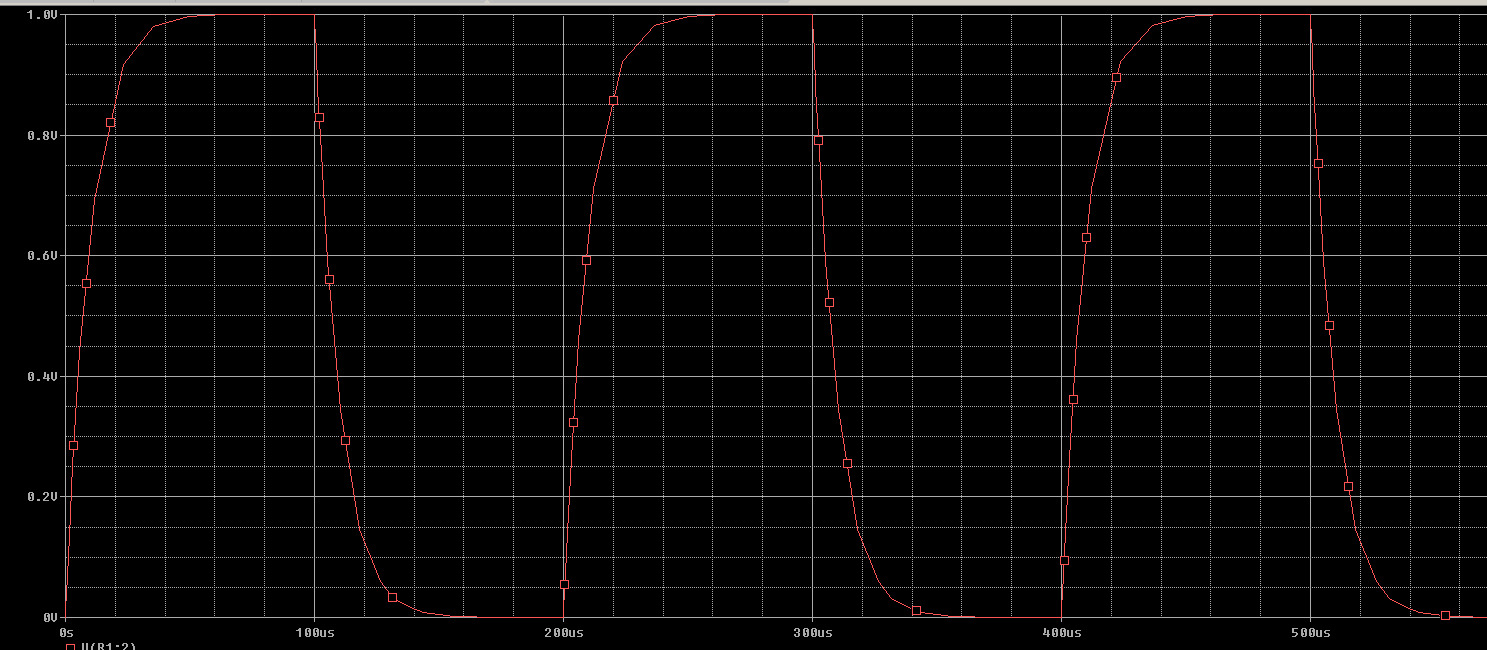
\includegraphics[width=110mm]{Pr0_1.jpeg}
		\caption{Simulació 1}
		\end{center}
	\end{figure}

	\section{Varies freqüencies diferents}

	Podem veure, tal i com esperavem ja que el circuit es passa-baixos, que al augmentar la frequencia la amplitud va disminuint.
	
	\begin{figure}[H]
		\begin{center}
		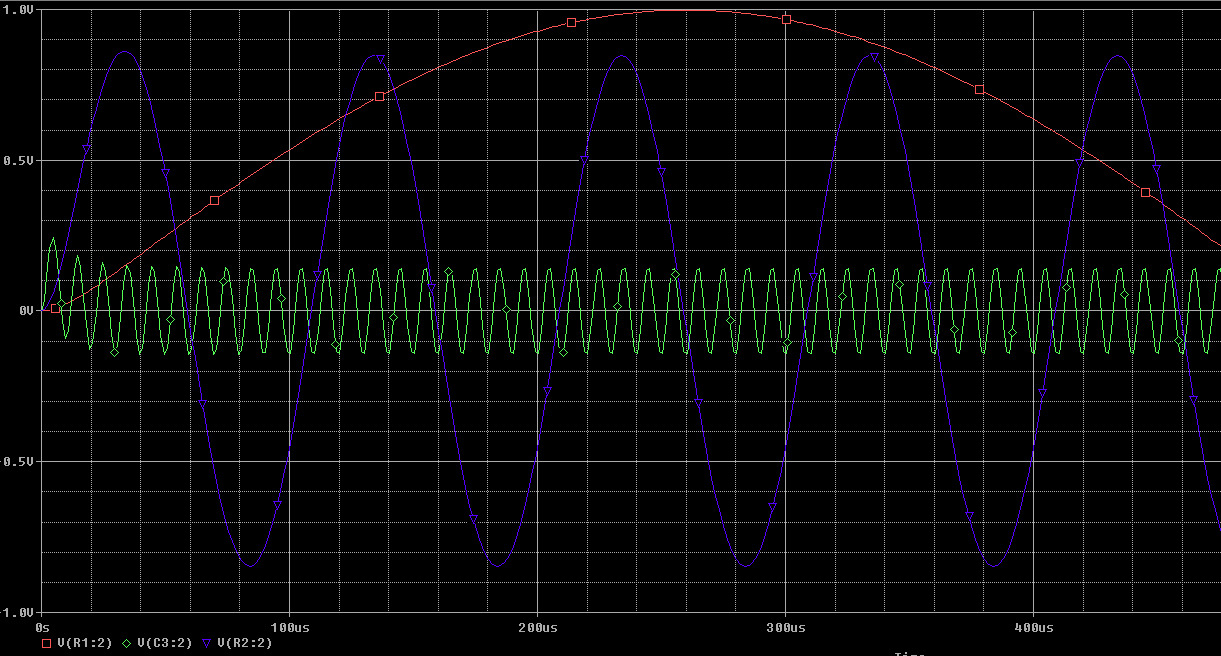
\includegraphics[width=110mm]{Pr0_2.jpeg}
		\caption{Simulació 2}
		\end{center}
	\end{figure}
	
	\section{Amplitud en funció de la frequencia}
	
	Podem veure aquí com disminueix l'amplitud en funció de la frequencia, confirmant-nos altre cop de que el filtre es passa-baixos.
	
	\begin{figure}[H]
		\begin{center}
		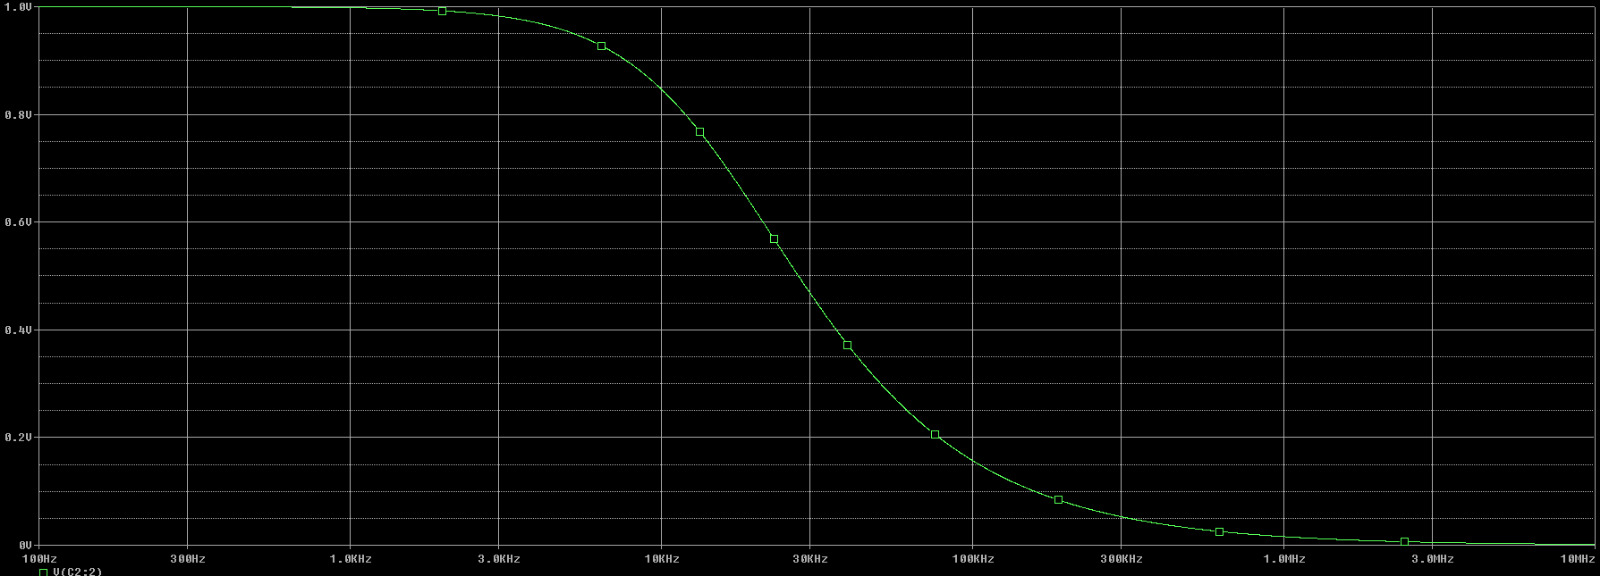
\includegraphics[width=110mm]{Pr0_3.jpeg}
		\caption{Simulació 3}
		\end{center}
	\end{figure}
	
	\section{Exercici 4}
	
	Repetim el mateix procediment amb un filtre passa alts com es el següent.

	\begin{figure}[H]
		\begin{center}
		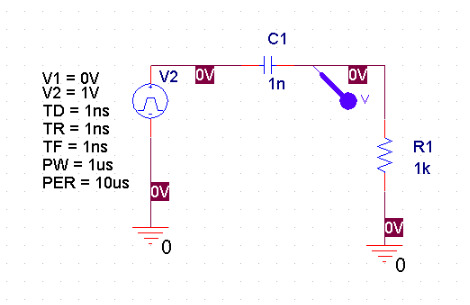
\includegraphics[width=110mm]{Pr0_circ.jpeg}
		\caption{Circuit passa alts}
		\end{center}
	\end{figure}
	
	\subsection{Pols rectangular}
	
	La sortida d'aquest circuit amb el pols rectangular proposat al exercici anterior es gairebe nula, ja que es un filtre passa altes i la frequencia del pols es molt baixa, així que he augmentat la frequencia i hem pogut obtenir la següent senyal, encara una mica atenuada.
	
	\begin{figure}[H]
		\begin{center}
		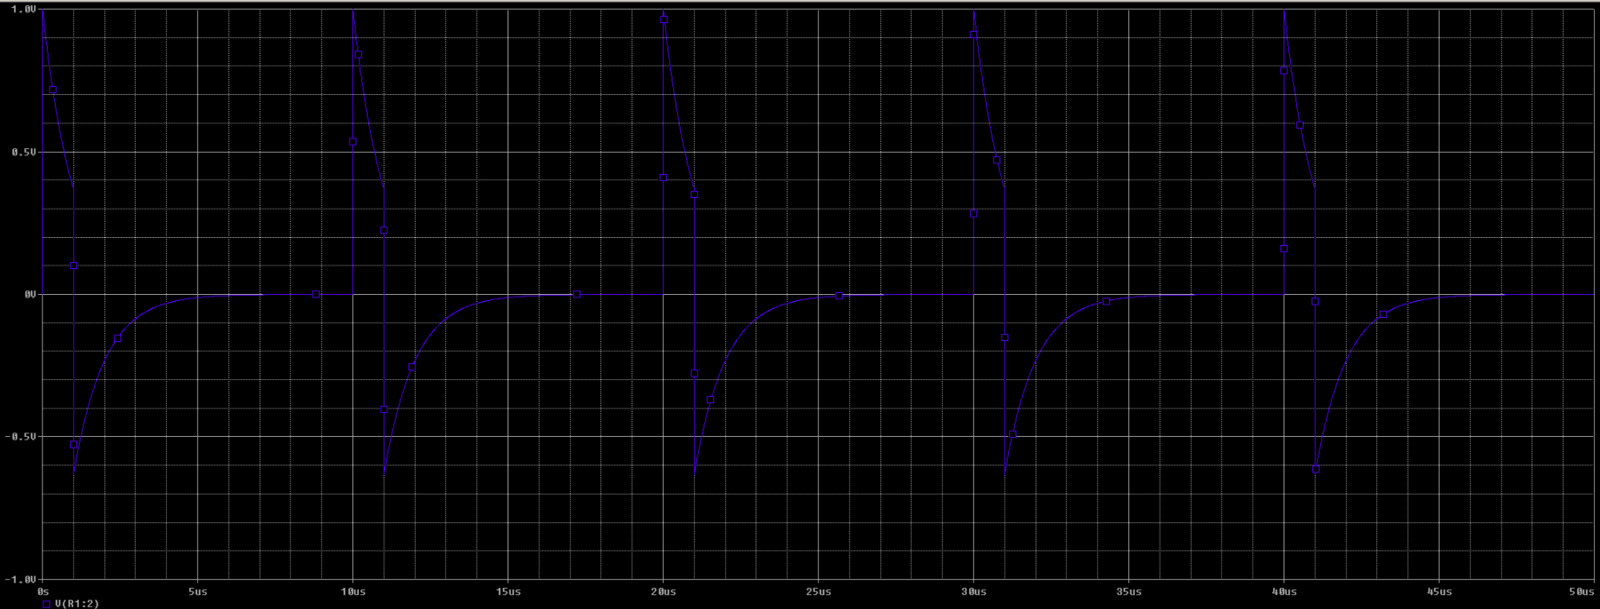
\includegraphics[width=110mm]{Pr0_4_1.jpeg}
		\caption{Circuit passa alts}
		\end{center}
	\end{figure}
	
	\subsection{Varies freqüencies diferents}
	
	Podem veure clarament que la frequencia mes elevada es la que conserva millor l'amplitud.
	
	\begin{figure}[H]
		\begin{center}
		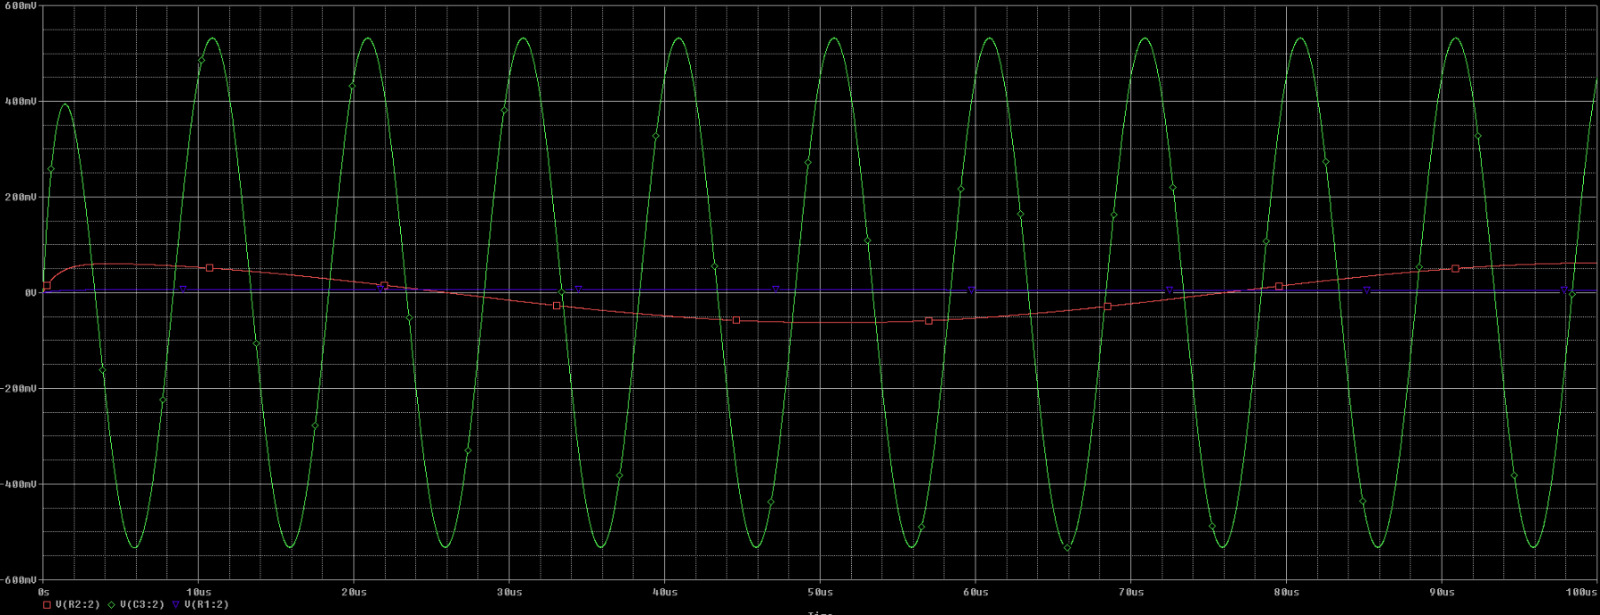
\includegraphics[width=110mm]{Pr0_4_2.jpeg}
		\caption{Circuit passa alts}
		\end{center}
	\end{figure}
	
	\subsection{Amplitud en funció de la frequencia}
	
	Finalment grafiquem la amplitud en funció de la frequencia cosa que ens confirma un altre cop que el filtre es passa altes.

	\begin{figure}[H]
		\begin{center}
		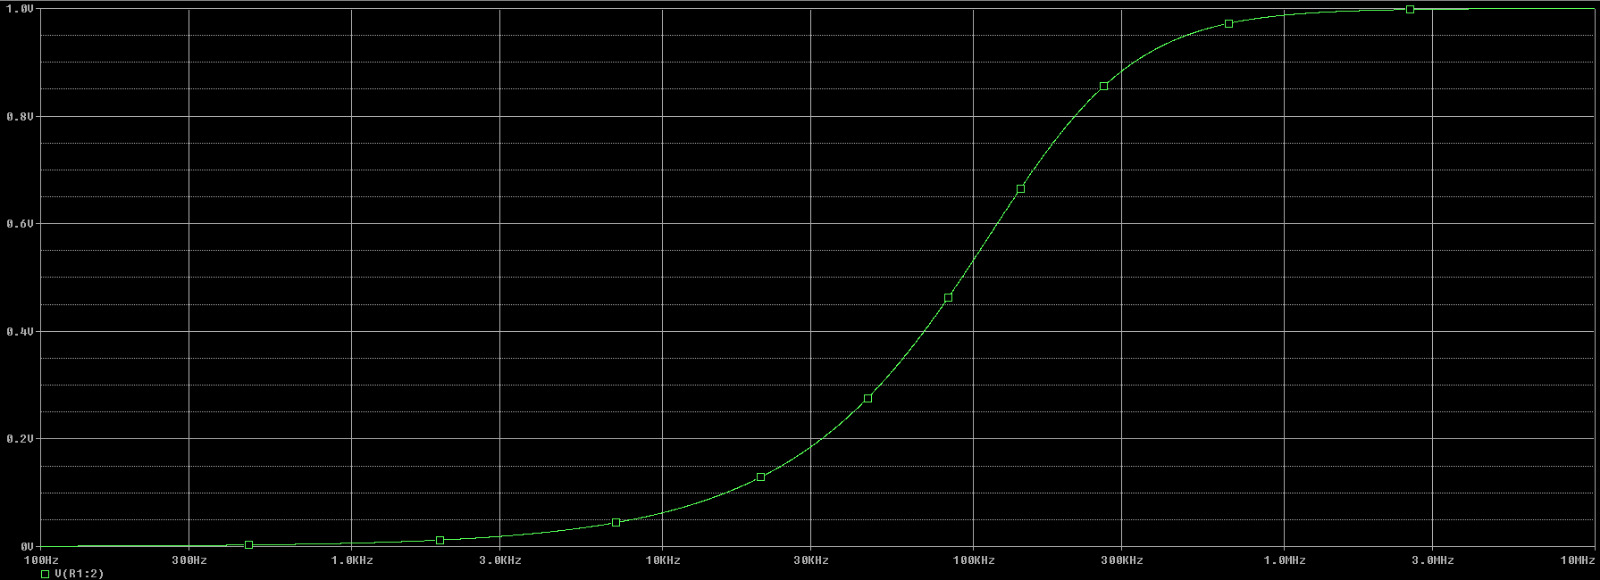
\includegraphics[width=110mm]{Pr0_4_3.jpeg}
		\caption{Circuit passa alts}
		\end{center}
	\end{figure}


\end{document}










